\section{แผนภาพยูสเคส (Use Case Diagram)}
\begin{figure}
    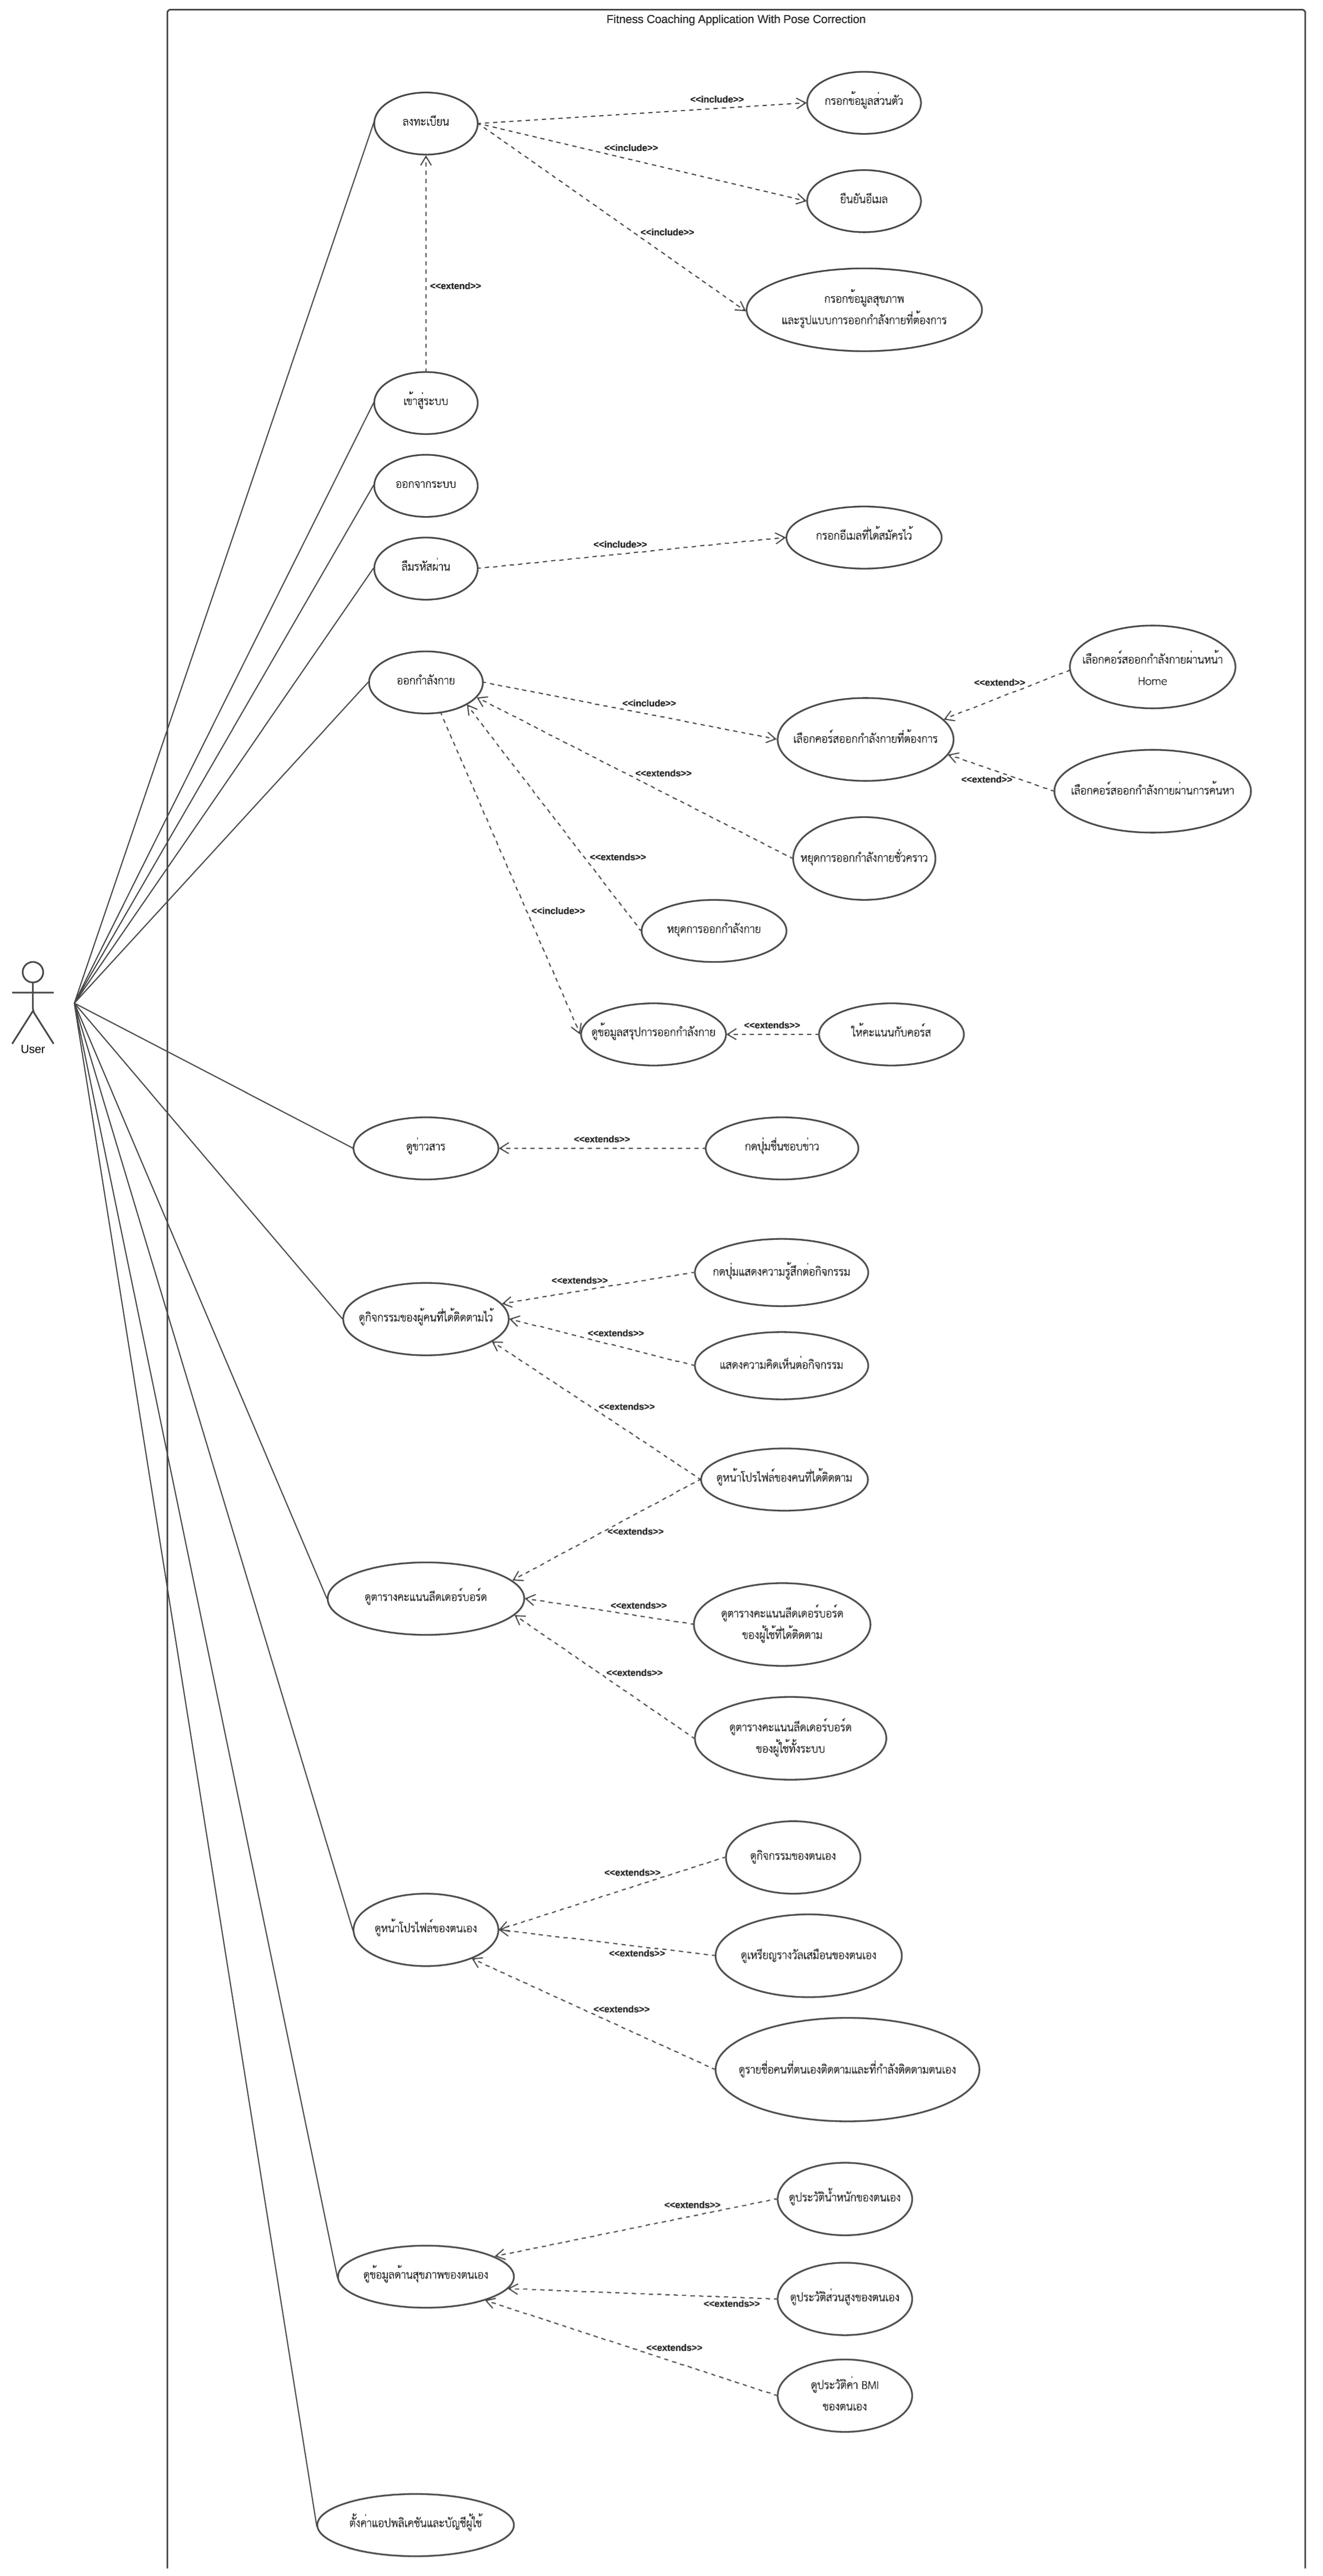
\includegraphics[height=\textheight - 3cm]{chapter_3/use case}
    \caption{แผนภาพยูสเคส}
\end{figure}
จากแผนภาพยูสเคสสามารถอธิบายได้ดังนี้
\begin{enumerate}
    \item ผู้ใช้สามารถลงทะเบียนเข้าใช้งานแอปพลิเคชันได้
    \item ผู้ใช้สามารถเข้าสู่ระบบได้
    \item ผู้ใช้สามารถออกจากระบบได้
    \item ผู้ใช้สามารถทำการกดลืมรหัสผ่านเพื่อตั้งค่ารหัสผ่านใหม่ได้
    \item ผู้ใช้สามารถเข้าสู่การออกกำลังกายได้
    \item ผู้ใช้สามารถดูข่าวสารของแอปพลิเคชันได้
    \item ผู้ใช้สามารถดูกิจกรรมของผู้คนที่ได้ติดตามไว้ได้
    \item ผู้ใช้สามารถดูตารางคะแนนลีดเดอร์บอร์ดได้
    \item ผู้ใช้สามารถดูหน้าโปรไฟล์ของตนเองได้
    \item ผู้ใช้สามารถดูข้อมูลด้านสุขภาพของตนเองได้
    \item ผู้ใช้สามารถตั้งค่าแอปพลิเคชันและตั้งค่าบัญชีผู้ใช้ได้
\end{enumerate}
\clearpage

\begin{table}
    \caption{รายละเอียด ลงทะเบียน}
    \begin{tabularx}{\textwidth}{ | >{\centering\bf} p{3cm} | X |}
        \hline
        Use Case: & ลงทะเบียน \\\hline
        Actor: & ผู้ใช้ \\\hline
        Main Flow: &
            \begin{enumerate}[table]
                \item ผู้ใช้ทำการกรอก email
                \item ผู้ใช้ทำการกรอก password ที่ต้องการ
                \item ผู้ใช้ทำการกรอก password เพื่อยืนยันอีกครั้ง
                \item ผู้ใช้ตรวจสอบการ verify email ที่ email ของตนเอง
                \item ผู้ใช้ทำการกรอก display name ที่ต้องการ
                \item ผู้ใช้ทำการเพิ่ม profile picture (สามารถข้ามได้)
            \end{enumerate}\\\hline
        Exception Flow: &
            \begin{enumerate}[table]
                \item กรณีผู้ใช้ทำการกรอก email ไม่ถูกต้องตามรูปแบบที่กำหนด แอปพลิเคชันจะแสดงข้อความว่า “Please enter a valid email”
                \item กรณีผู้ใช้ทำการกรอก password ทั้งสองช่องไม่ตรงกัน แอปพลิเคชันจะแสดงข้อความว่า “Please confirm your password”
                \item กรณีผู้ใช้ทำการกรอก password ไม่ถูกต้องตามที่เงื่อนไขกำหนด แอปพลิเคชันจะแสดงข้อความว่า “Your password must be at least 6 characters long. Please try another.”
                \item กรณีผู้ใช้ทำการกรอก display name ที่ซ้ำกันในระบบ แอปพลิเคชันจะแสดงข้อความ “This display name is already exist.”
            \end{enumerate}\\\hline
    \end{tabularx}
\end{table}


\begin{table}
    \caption{รายละเอียด เข้าสู่ระบบ}
    \begin{tabularx}{\textwidth}{ | >{\centering\bf} p{3cm} | X |}
        \hline
        Use Case: & เข้าสู่ระบบ \\\hline
        Actor: & ผู้ใช้ \\\hline
        Pre-Condition: &
        \begin{enumerate}[table]
            \item ผู้ใช้ได้เชื่อมต่ออินเทอร์เน็ต
            \item ผู้ใช้ต้องมีบัญชีผู้ใช้อยู่ในระบบ
        \end{enumerate} \\\hline
        
        Main Flow: & 
        \begin{enumerate}[table]
            \item ผู้ใช้กรอก email และ password
            \item ผู้ใช้ทำการกดปุ่มเข้าสู่ระบบ
        \end{enumerate}\\\hline
        Exception Flow: & 
        \begin{enumerate}[table]
            \item กรณีผู้ใช้ทำการกรอก email ไม่ถูกต้องตามรูปแบบที่กำหนด แอปพลิเคชันจะแสดงข้อความว่า “Please enter a valid email”
        \end{enumerate}\\\hline
    \end{tabularx}
\end{table}


\begin{table}
    \caption{รายละเอียด ออกจากระบบ}
    \begin{tabularx}{\textwidth}{ | >{\centering\bf} p{3cm} | X |}
        \hline
        Use Case: & ออกจากระบบ \\\hline
        Actor: & ผู้ใช้ \\\hline
        Pre-Condition: &
        \begin{enumerate}[table]
            \item ผู้ใช้ได้เข้าสู่ระบบเรียบร้อยแล้ว
        \end{enumerate} \\\hline
        
        Main Flow: & 
        \begin{enumerate}[table]
            \item ผู้ใช้กดปุ่มออกจากระบบ
        \end{enumerate}\\\hline
    \end{tabularx}
\end{table}

\begin{table}
    \caption{รายละเอียด ลืมรหัสผ่าน}
    \begin{tabularx}{\textwidth}{ | >{\centering\bf} p{3cm} | X |}
        \hline
        Use Case: & ลืมรหัสผ่าน \\\hline
        Actor: & ผู้ใช้ \\\hline
        Pre-Condition: &
        \begin{enumerate}[table]
            \item ผู้ใช้ได้เชื่อมต่ออินเทอร์เน็ต
            \item ผู้ใช้ต้องมีบัญชีผู้ใช้อยู่ในระบบ
        \end{enumerate} \\\hline
        
        Main Flow: & 
        \begin{enumerate}[table]
            \item ผู้ใช้กรอก email ที่ได้ทำการลงทะเบียนไว้
            \item แอปพลิเคชันส่งอีเมลเพื่อ reset รหัสผ่านไปยังผู้ใช้
            \item ผู้ใช้คลิกลิงก์เพื่อกำหนดรหัสผ่านใหม่
        \end{enumerate}\\\hline
        Exception Flow: & 
        \begin{enumerate}[table]
            \item กรณีผู้ใช้ทำการกรอก password ทั้งสองช่องไม่ตรงกัน แอปพลิเคชันจะแสดงข้อความว่า “Please confirm your password”
            \item กรณีผู้ใช้ทำการกรอก password ไม่ถูกต้องตามที่เงื่อนไขกำหนด แอปพลิเคชันจะแสดงข้อความว่า “Your password must be at least 6 characters long. Please try another.”
        \end{enumerate}\\\hline
    \end{tabularx}
\end{table}


\begin{table}
    \caption{รายละเอียด ออกกำลังกาย}
    \begin{tabularx}{\textwidth}{ | >{\centering\bf} p{3cm} | X |}
        \hline
        Use Case: & ออกกำลังกาย \\\hline
        Actor: & ผู้ใช้ \\\hline
        Pre-Condition: &
        \begin{enumerate}[table]
            \item ผู้ใช้ได้เข้าสู่ระบบเรียบร้อยแล้ว
        \end{enumerate} \\\hline
        
        Main Flow: & 
        \begin{enumerate}[table]
            \item ผู้ใช้กดเข้าหน้าหลักหรือค้นหาคอร์สออกกำลังกายเพื่อเลือกคอร์สออกกำลังกาย
            \item ผู้ใช้กดเลือกคอร์สออกกำลังกายที่ต้องการ
            \item ผู้ใช้วางโทรศัพท์มือถือ โดยให้กล้องหน้ามองเห็นร่างกายของผู้ใช้
            \item ผู้ใช้ออกกำลังกาย โดยทำตามท่าทางที่ทางแอปพลิเคชันได้สอนไว้
            \item ในระหว่างการออกกำลังกาย ผู้ใช้สามารถหยุดการออกกำลังกายชั่วคราว
            \item ในระหว่างการออกกำลังกาย ผู้ใช้สามารถหยุดการออกกำลังกาย
            \item เมื่อจบการออกกำลังกาย แอปพลิเคชันจะแสดงข้อมูลสรุปการออกกำลังกาย
            \item ผู้ใช้ให้คะแนนกับคอร์สออกกำลังกายที่ได้ออกไป
        \end{enumerate}\\\hline
        Exception Flow: & 
        \begin{enumerate}[table]
            \item เมื่อผู้ใช้ออกกำลังกายไม่ถูกต้อง แอปพลิเคชันจะมีเสียงแจ้งผู้ใช้ว่ากำลังออกกำลังกายไม่ถูกต้อง
        \end{enumerate}\\\hline
    \end{tabularx}
\end{table}


\begin{table}
    \caption{รายละเอียด หยุดการออกกำลังกายชั่วคราว}
    \begin{tabularx}{\textwidth}{ | >{\centering\bf} p{3cm} | X |}
        \hline
        Use Case: & หยุดการออกกำลังกายชั่วคราว \\\hline
        Actor: & ผู้ใช้ \\\hline
        Pre-Condition: &
        \begin{enumerate}[table]
            \item ผู้ใช้ได้เข้าสู่ระบบเรียบร้อยแล้ว
            \item ผู้ใช้อยู่ในหน้าการออกกำลังกาย
        \end{enumerate} \\\hline
        
        Main Flow: & 
        \begin{enumerate}[table]
            \item ผู้ใช้กดปุ่ม Pause เพื่อหยุดการออกกำลังกายชั่วคราว
            \item แอปพลิเคชันหยุดการจับเวลาการออกกำลังกายชั่วคราว
            \item ผู้ใช้กดปุ่ม Resume เพื่อเริ่มการออกกำลังกายต่อ
        \end{enumerate}\\\hline
    \end{tabularx}
\end{table}

\begin{table}
    \caption{รายละเอียด หยุดการออกกำลังกาย}
    \begin{tabularx}{\textwidth}{ | >{\centering\bf} p{3cm} | X |}
        \hline
        Use Case: & หยุดการออกกำลังกาย \\\hline
        Actor: & ผู้ใช้ \\\hline
        Pre-Condition: &
        \begin{enumerate}[table]
            \item ผู้ใช้ได้เข้าสู่ระบบเรียบร้อยแล้ว
            \item ผู้ใช้อยู่ในหน้าการออกกำลังกาย
        \end{enumerate} \\\hline
        
        Main Flow: & 
        \begin{enumerate}[table]
            \item ผู้ใช้กดปุ่ม Stop เพื่อหยุดการออกกำลังกาย หรือเมื่อผู้ใช้ออกกำลังกายเสร็จสิ้น
            \item แอปพลิเคชันหยุดการออกกำลังกาย
        \end{enumerate}\\\hline
    \end{tabularx}
\end{table}

\begin{table}
    \caption{รายละเอียด ดูข่าวสาร}
    \begin{tabularx}{\textwidth}{ | >{\centering\bf} p{3cm} | X |}
        \hline
        Use Case: & ดูข่าวสาร \\\hline
        Actor: & ผู้ใช้ \\\hline
        Pre-Condition: &
        \begin{enumerate}[table]
            \item ผู้ใช้เข้าสู่ระบบเรียบร้อยแล้ว
        \end{enumerate} \\\hline
        
        Main Flow: & 
        \begin{enumerate}[table]
            \item ผู้ใช้กดปุ่มเลือกเข้าสู่หน้า News
            \item แอปพลิเคชันแสดงข้อมูลข่าวสาร
            \item ผู้ใช้เลือกอ่านข้อมูลข่าวสารที่เกี่ยวข้องกับการออกกำลังกาย ตามต้องการ
        \end{enumerate}\\\hline
    \end{tabularx}
\end{table}


\begin{table}
    \caption{รายละเอียด กดปุ่มชื่นชอบข่าว}
    \begin{tabularx}{\textwidth}{ | >{\centering\bf} p{3cm} | X |}
        \hline
        Use Case: & ดูข่าวสาร \\\hline
        Actor: & ผู้ใช้ \\\hline
        Pre-Condition: &
        \begin{enumerate}[table]
            \item ผู้ใช้ได้เข้าสู่ระบบเรียบร้อยแล้ว
            \item ผู้ใช้อยู่หน้าอ่านข้อมูลข่าวสาร          
        \end{enumerate} \\\hline
        
        Main Flow: & 
        \begin{enumerate}[table]
            \item ผู้ใช้ดูข้อมูลข่าวสาร
            \item ผู้ใช้กดปุ่มชื่นชอบข่าวสาร      
        \end{enumerate}\\\hline
    \end{tabularx}
\end{table}


\begin{table}
    \caption{รายละเอียด ดูกิจกรรมของผู้คนที่ได้ติดตามไว้}
    \begin{tabularx}{\textwidth}{ | >{\centering\bf} p{3cm} | X |}
        \hline
        Use Case: & ดูกิจกรรมของผู้คนที่ได้ติดตามไว้ \\\hline
        Actor: & ผู้ใช้ \\\hline
        Pre-Condition: &
        \begin{enumerate}[table]
            \item ผู้ใช้เข้าสู่ระบบเรียบร้อยแล้ว         
        \end{enumerate} \\\hline
        
        Main Flow: & 
        \begin{enumerate}[table]
            \item ผู้ใช้กดปุ่มเลือกเข้าสู่หน้า Activity
            \item ผู้ใช้เลือกดูกิจกรรมของผู้ใช้ที่ได้ติดตามไว้
            \item ผู้ใช้สามารถกดปุ่มแสดงความรู้สึกต่อกิจกรรม
            \item ผู้ใช้สามารถแสดงความคิดเห็นต่อกิจกรรม
            \item ผู้ใช้สามารถดูหน้าโปรไฟล์ของผู้ใช้ที่ได้ติดตามไว้
        \end{enumerate}\\\hline
    \end{tabularx}
\end{table}


\begin{table}
    \caption{รายละเอียด กดปุ่มแสดงความรู้สึกต่อกิจกรรม}
    \begin{tabularx}{\textwidth}{ | >{\centering\bf} p{3cm} | X |}
        \hline
        Use Case: & กดปุ่มแสดงความรู้สึกต่อกิจกรรม \\\hline
        Actor: & ผู้ใช้ \\\hline
        Pre-Condition: &
        \begin{enumerate}[table]
            \item ผู้ใช้ได้เข้าสู่ระบบเรียบร้อยแล้ว
            \item ผู้ใช้เลือกดูกิจกรรมของผู้ใช้ที่ได้ติดตามไว้
                   
        \end{enumerate} \\\hline
        
        Main Flow: & 
        \begin{enumerate}[table]
            \item ผู้ใช้กดปุ่มแสดงความรู้สึกต่อกิจกรรม
        \end{enumerate}\\\hline
    \end{tabularx}
\end{table}


\begin{table}
    \caption{รายละเอียด แสดงความคิดเห็นต่อกิจกรรม}
    \begin{tabularx}{\textwidth}{ | >{\centering\bf} p{3cm} | X |}
        \hline
        Use Case: & แสดงความคิดเห็นต่อกิจกรรม \\\hline
        Actor: & ผู้ใช้ \\\hline
        Pre-Condition: &
        \begin{enumerate}[table]
            \item ผู้ใช้ได้เข้าสู่ระบบเรียบร้อยแล้ว
            \item ผู้ใช้เลือกดูกิจกรรมของผู้ใช้ที่ได้ติดตามไว้      
        \end{enumerate} \\\hline
        
        Main Flow: & 
        \begin{enumerate}[table]
            \item ผู้ใช้กดแสดงความคิดเห็นต่อกิจกรรม
        \end{enumerate}\\\hline
    \end{tabularx}
\end{table}



\begin{table}
    \caption{รายละเอียด ดูตารางคะแนนลีดเดอร์บอร์ด}
    \begin{tabularx}{\textwidth}{ | >{\centering\bf} p{3cm} | X |}
        \hline
        Use Case: & ดูตารางคะแนนลีดเดอร์บอร์ด \\\hline
        Actor: & ผู้ใช้ \\\hline
        Pre-Condition: &
        \begin{enumerate}[table]
            \item ผู้ใช้ได้เข้าสู่ระบบเรียบร้อยแล้ว
            \item ผู้ใช้อยู่ในหน้า Activity
        \end{enumerate} \\\hline
        
        Main Flow: & 
        \begin{enumerate}[table]
            \item ผู้ใช้กดปุ่ม Leaderboard
            \item แอปพลิเคชันแสดงตารางคะแนนลีดเดอร์บอร์ด
            \item ผู้ใช้กดปุ่มเพื่อแสดงตารางคะแนนลีดเดอร์บอร์ดโดยจำแนกตามกลุ่มผู้ใช้ที่ได้ติดตามไว้ และกลุ่มผู้ใช้ทั้งระบบ
            \item ผู้ใช้สามารถกดดูหน้าโปรไฟล์ของผู้ใช้ที่ได้ติดตามไว้
        \end{enumerate}\\\hline
    \end{tabularx}
\end{table}



\begin{table}
    \caption{รายละเอียด ดูตารางคะแนนลีดเดอร์บอร์ดของผู้ใช้ที่ได้ติดตาม}
    \begin{tabularx}{\textwidth}{ | >{\centering\bf} p{3cm} | X |}
        \hline
        Use Case: & ดูตารางคะแนนลีดเดอร์บอร์ดของผู้ใช้ที่ได้ติดตาม \\\hline
        Actor: & ผู้ใช้ \\\hline
        Pre-Condition: &
        \begin{enumerate}[table]
            \item ผู้ใช้ได้เข้าสู่ระบบเรียบร้อยแล้ว
            \item ผู้ใช้อยู่ในหน้าแสดงตารางคะแนนลีดเดอร์บอร์ด         
        \end{enumerate} \\\hline
        
        Main Flow: & 
        \begin{enumerate}[table]
            \item ผู้ใช้กดปุ่มแสดงตารางคะแนนลีดเดอร์บอร์ดโดยจำแนกตามกลุ่มผู้ใช้ที่ได้ติดตามไว้
        \end{enumerate}\\\hline
    \end{tabularx}
\end{table}


\begin{table}
    \caption{รายละเอียด ดูตารางคะแนนลีดเดอร์บอร์ดของผู้ใช้ทั้งระบบ}
    \begin{tabularx}{\textwidth}{ | >{\centering\bf} p{3cm} | X |}
        \hline
        Use Case: & ดูตารางคะแนนลีดเดอร์บอร์ดของผู้ใช้ทั้งระบบ \\\hline
        Actor: & ผู้ใช้ \\\hline
        Pre-Condition: &
        \begin{enumerate}[table]
            \item ผู้ใช้ได้เข้าสู่ระบบเรียบร้อยแล้ว
            \item ผู้ใช้อยู่ในหน้าแสดงตารางคะแนนลีดเดอร์บอร์ด            
        \end{enumerate} \\\hline
        
        Main Flow: & 
        \begin{enumerate}[table]
            \item ผู้ใช้กดปุ่มแสดงตารางคะแนนลีดเดอร์บอร์ดโดยจำแนกตามกลุ่มผู้ใช้ทั้งระบบ
        \end{enumerate}\\\hline
    \end{tabularx}
\end{table}



\begin{table}
    \caption{รายละเอียด ดูหน้าโปรไฟล์ของตนเอง}
    \begin{tabularx}{\textwidth}{ | >{\centering\bf} p{3cm} | X |}
        \hline
        Use Case: & ดูหน้าโปรไฟล์ของตนเอง \\\hline
        Actor: & ผู้ใช้ \\\hline
        Pre-Condition: &
        \begin{enumerate}[table]
            \item ผู้ใช้ได้เข้าสู่ระบบเรียบร้อยแล้ว         
        \end{enumerate} \\\hline
        
        Main Flow: & 
        \begin{enumerate}[table]
            \item ผู้ใช้กดปุ่มเลือกเข้าสู่หน้า Profile
            \item แอปพลิเคชันแสดงข้อมูลสรุปของผู้ใช้
            \item ผู้ใช้ตรวจสอบกิจกรรมของตนเอง
            \item ผู้ใช้ตรวจสอบเหรียญรางวัลเสมือนของตนเอง
            \item ผู้ใช้ตรวจสอบรายชื่อการติดตามกับผู้ใช้อื่น
        \end{enumerate}\\\hline
    \end{tabularx}
\end{table}


\begin{table}
    \caption{รายละเอียด ดูกิจกรรมของตนเอง}
    \begin{tabularx}{\textwidth}{ | >{\centering\bf} p{3cm} | X |}
        \hline
        Use Case: & ดูกิจกรรมของตนเอง \\\hline
        Actor: & ผู้ใช้ \\\hline
        Pre-Condition: &
        \begin{enumerate}[table]
            \item ผู้ใช้ได้เข้าสู่ระบบเรียบร้อยแล้ว
            \item ผู้ใช้อยู่ในหน้า Profile 
        \end{enumerate} \\\hline
        
        Main Flow: & 
        \begin{enumerate}[table]
            \item ผู้ใช้กดปุ่มเลือกเข้าสู่หน้า Profile
            \item แอปพลิเคชันแสดงข้อมูลสรุปของผู้ใช้
            \item ผู้ใช้ตรวจสอบกิจกรรมของตนเอง
            \item ผู้ใช้ตรวจสอบเหรียญรางวัลเสมือนของตนเอง
            \item ผู้ใช้ตรวจสอบรายชื่อการติดตามกับผู้ใช้อื่น
        \end{enumerate}\\\hline
    \end{tabularx}
\end{table}


\begin{table}
    \caption{รายละเอียด ดูเหรียญรางวัลเสมือนของตนเอง}
    \begin{tabularx}{\textwidth}{ | >{\centering\bf} p{3cm} | X |}
        \hline
        Use Case: & ดูเหรียญรางวัลเสมือนของตนเอง \\\hline
        Actor: & ผู้ใช้ \\\hline
        Pre-Condition: &
        \begin{enumerate}[table]
            \item ผู้ใช้ได้เข้าสู่ระบบเรียบร้อยแล้ว
            \item ผู้ใช้อยู่ในหน้า Profile
            
        \end{enumerate} \\\hline
        
        Main Flow: & 
        \begin{enumerate}[table]
            \item ผู้ใช้กดปุ่มแสดงเหรียญรางวัลเสมือนของตนเอง
            \item ผู้ใช้ตรวจสอบเหรียญรางวัลเสมือนของตนเอง
        \end{enumerate}\\\hline
    \end{tabularx}
\end{table}


\begin{table}
    \caption{รายละเอียด ดูรายชื่อคนที่ตนเองติดตามและที่กำลังติดตามตนเอง}
    \begin{tabularx}{\textwidth}{ | >{\centering\bf} p{3cm} | X |}
        \hline
        Use Case: & ดูรายชื่อคนที่ตนเองติดตามและที่กำลังติดตามตนเอง \\\hline
        Actor: & ผู้ใช้ \\\hline
        Pre-Condition: &
        \begin{enumerate}[table]
            \item ผู้ใช้ได้เข้าสู่ระบบเรียบร้อยแล้ว
            \item ผู้ใช้อยู่ในหน้า Profile
        \end{enumerate} \\\hline
        
        Main Flow: & 
        \begin{enumerate}[table]
            \item ผู้ใช้กดข้อความ Follower เพื่อตรวจสอบรายชื่อคนที่กำลังติดตามตนเอง
            \item ผู้ใช้กดข้อความ Following เพื่อตรวจสอบรายชื่อคนที่ตนเองติดตาม
            \item แอปพลิเคชันแสดงรายชื่อคนที่ตนเองติดตามและที่กำลังติดตามตนเอง
            \item ผู้ใช้ตรวจสอบรายชื่อคนที่ตนเองติดตามและที่กำลังติดตามตนเอง
        \end{enumerate} \\\hline
    \end{tabularx}
\end{table}


\begin{table}
    \caption{รายละเอียด ดูข้อมูลด้านสุขภาพของตนเอง}
    \begin{tabularx}{\textwidth}{ | >{\centering\bf} p{3cm} | X |}
        \hline
        Use Case: & ดูข้อมูลด้านสุขภาพของตนเอง \\\hline
        Actor: & ผู้ใช้ \\\hline
        Pre-Condition: &
        \begin{enumerate}[table]
            \item ผู้ใช้ได้เข้าสู่ระบบเรียบร้อยแล้ว
            \item ผู้ใช้อยู่ในหน้า Profile            
        \end{enumerate} \\\hline
        
        Main Flow: & 
        \begin{enumerate}[table]
            \item ผู้ใช้กดปุ่ม Health Stats
            \item แอปพลิเคชันแสดงหน้า Health Stats ซึ่งแสดงข้อมูลด้านสุขภาพ (จำนวนนาทีการออกกำลังกาย, น้ำหนัก, ส่วนสูง, ค่า BMI) ของตนเอง
            \item ผู้ใช้ตรวจสอบข้อมูลด้านสุขภาพของตนเอง  
        \end{enumerate}\\\hline
    \end{tabularx}
\end{table}


\begin{table}
    \caption{รายละเอียด ดูประวัติน้ำหนักของตนเอง}
    \begin{tabularx}{\textwidth}{ | >{\centering\bf} p{3cm} | X |}
        \hline
        Use Case: & ดูประวัติน้ำหนักของตนเอง \\\hline
        Actor: & ผู้ใช้ \\\hline
        Pre-Condition: &
        \begin{enumerate}[table]
            \item ผู้ใช้ได้เข้าสู่ระบบเรียบร้อยแล้ว
            \item ผู้ใช้อยู่ในหน้า Health Stats          
        \end{enumerate} \\\hline
        
        Main Flow: & 
        \begin{enumerate}[table]
            \item ผู้ใช้กดปุ่ม Weight
            \item แอปพลิเคชันแสดงข้อมูลสถิติของค่าน้ำหนักของผู้ใช้ที่ได้บันทึกไว้ โดยแสดงเป็นกราฟเส้นและค่าที่ได้บันทึกไว้
            \item ผู้ใช้ตรวจสอบสถิติค่าน้ำหนักของตนเอง
        \end{enumerate}\\\hline
    \end{tabularx}
\end{table}



\begin{table}
    \caption{รายละเอียด ดูประวัติส่วนสูงของตนเอง}
    \begin{tabularx}{\textwidth}{ | >{\centering\bf} p{3cm} | X |}
        \hline
        Use Case: & ดูประวัติส่วนสูงของตนเอง \\\hline
        Actor: & ผู้ใช้ \\\hline
        Pre-Condition: &
        \begin{enumerate}[table]
            \item ผู้ใช้ได้เข้าสู่ระบบเรียบร้อยแล้ว
            \item ผู้ใช้อยู่ในหน้า Health Stats          
        \end{enumerate} \\\hline
        
        Main Flow: & 
        \begin{enumerate}[table]
            \item ผู้ใช้กดปุ่ม Height
            \item แอปพลิเคชันแสดงข้อมูลสถิติของค่าส่วนสูงของผู้ใช้ที่ได้บันทึกไว้ โดยแสดงเป็นกราฟเส้นและค่าที่ได้บันทึกไว้
            \item ผู้ใช้ตรวจสอบสถิติค่าส่วนสูงของตนเอง   
        \end{enumerate}\\\hline
    \end{tabularx}
\end{table}


\begin{table}
    \caption{รายละเอียด ดูประวัติค่า BMI ของตนเอง}
    \begin{tabularx}{\textwidth}{ | >{\centering\bf} p{3cm} | X |}
        \hline
        Use Case: & ดูประวัติค่า BMI ของตนเอง \\\hline
        Actor: & ผู้ใช้ \\\hline
        Pre-Condition: &
        \begin{enumerate}[table]
            \item ผู้ใช้ได้เข้าสู่ระบบเรียบร้อยแล้ว
            \item ผู้ใช้อยู่ในหน้า Health Stats
        \end{enumerate} \\\hline
        
        Main Flow: & 
        \begin{enumerate}[table]
            \item ผู้ใช้กดปุ่ม BMI
            \item แอปพลิเคชันแสดงข้อมูลสถิติของค่า BMI ของผู้ใช้ที่แอปพลิเคชันคำนวณมาจากค่าน้ำหนักและส่วนสูงที่ผู้ใช้ได้บันทึกไว้
            \item ผู้ใช้ตรวจสอบสถิติค่า BMI ของตนเอง
        \end{enumerate}\\\hline
    \end{tabularx}
\end{table}



\begin{table}
    \caption{รายละเอียด ตั้งค่าแอปพลิเคชันและบัญชีผู้ใช้}
    \begin{tabularx}{\textwidth}{ | >{\centering\bf} p{3cm} | X |}
        \hline
        Use Case: & ตั้งค่าแอปพลิเคชันและบัญชีผู้ใช้ \\\hline
        Actor: & ผู้ใช้ \\\hline
        Pre-Condition: &
        \begin{enumerate}[table]
            \item ผู้ใช้ได้เข้าสู่ระบบเรียบร้อยแล้ว
            \item ผู้ใช้อยู่ในหน้า Profile            
        \end{enumerate} \\\hline
        
        Main Flow: & 
        \begin{enumerate}[table]
            \item ผู้ใช้กดปุ่ม Settings
            \item แอปพลิเคชันแสดงหน้า Settings ในการตั้งค่าแอปพลิเคชันและบัญชีผู้ใช้
            \item ผู้ใช้ตรวจสอบการตั้งค่าแอปพลิเคชันและบัญชีผู้ใช้
            \item ผู้ใช้กำหนดค่าของการตั้งค่าแอปพลิเคชันและบัญชีผู้ใช้            
        \end{enumerate}\\\hline
    \end{tabularx}
\end{table}
\clearpage